% DAFN23 - Robotics - Lecture 1
% Roberto Masocco <roberto.masocco@uniroma2.it>
% May 14, 2023

\documentclass[aspectratio=169]{beamer}

% Slides layout
\usepackage[
    title={Roboticist 101},
    subtitle={Software and middleware for robotics},
    event={DAFN},
    author={Roberto Masocco},
    longauthor={Roberto Masocco},
    email={roberto.masocco@uniroma2.it},
    institute={Tor Vergata},
    longinstitute={University of Rome Tor Vergata},
    department={Department of Civil Engineering and Computer Science Engineering},
    researchgroup={},
    date={May 17, 2023}
]{utvengbeamer}

% Code listings settings
\usepackage[nomath]{lmodern}
\definecolor{codegreen}{rgb}{0 0.5 0}
\definecolor{codered}{rgb}{1 0 0}
\definecolor{codeocher}{rgb}{0.8 0.47 0.13}
\usepackage{listings}
\lstdefinestyle{beamer}{
    basicstyle=\ttfamily\small,
    commentstyle=\color{codegreen},
    breakatwhitespace=false,
    captionpos=b,
    frame=lines,
    keepspaces=true,
    keywordstyle=\color{codered}\bfseries,
    numbers=left,
    numbersep=5pt,
    numberstyle=\footnotesize,
    showspaces=false,
    showstringspaces=false,
    showtabs=false,
    stringstyle=\color{codeocher},
    tabsize=2
}
\lstset{style=beamer}
\lstdefinelanguage{Dockerfile}{
  alsoletter={[, ], _, /},
  morecomment=[l][\color{codegreen}]{\#},
  morekeywords={FROM, RUN, ADD, COPY, LABEL, ENV, ARG, CMD}
}
\lstdefinelanguage{compose}{
  alsoletter={:, -, /},
  morecomment=[l][\color{codegreen}]{\#},
  morekeywords={services:, build:, context:, network_mode:, args:, environment:, command:, volumes:, image:, -}
}

\usepackage{hyperref}
\usepackage{wasysym}

\begin{document}

% --- Title page ---
\frame{\titlepage}

% --- Table of contents ---
\begin{frame}
\frametitle{Roadmap}
\tableofcontents
\end{frame}

% --- Section 1 ---
% Section 1 - Introduction
% Roberto Masocco <roberto.masocco@uniroma2.it>
% May 14, 2023

% ### Introduction ###
\section{Introduction}
\graphicspath{{figs/section1/}}

% --- Information ---
\begin{frame}{Information}
	\begin{itemize}
		\item \textbg{Calendar}: from May 17 to June 14, 2023
		\item \textbg{Topics} (both with practical examples):
		      \begin{enumerate}
			      \item Middleware for robotics
			      \item 3D printing basics (with Simone Mattogno)
		      \end{enumerate}
		\item \textbg{Materials} (for my part):
		      \begin{itemize}
			      \item Code repository: \href{https://github.com/IntelligentSystemsLabUTV/ros2-examples}{\color{blue}\underline{github.com/ros2-examples}} (\texttt{humble} branch)
			      \item Lectures: \href{https://github.com/stars/robmasocco/lists/lectures}{\color{blue}\underline{github.com/robmasocco}}, Teams directory (this lecture is \href{https://github.com/robmasocco/DAFN23_Robotics_1}{\color{blue}\underline{here}})
		      \end{itemize}
		\item \textbg{Useful background} (for my part):
		      \begin{itemize}
			      \item Basics of C and Python programming
			      \item Basics of Git workflow (check out \href{https://www.atlassian.com/git/tutorials/what-is-git}{\color{blue}\underline{this tutorial}} by Atlassian)
			      \item Everyday Linux commands and a Unix-like system
		      \end{itemize}
		      \visible<2>{
		\item \textbg{Exam}: ... ask Prof. Carnevale \smiley
		      }
	\end{itemize}
\end{frame}

% --- Program ---
\begin{frame}{Program}{Middleware for robotics}
	\begin{enumerate}
		\item Roboticist 101 - Software and middleware for robotics
		\item ROS 2 - Workflow and basic communication
		\item ROS 2 - Advanced communication
		\item ROS 2 - Node configuration
		\item ROS 2 - Sensor sampling and image processing
		\item ROS 2 - Interfacing with the data space
		\item microROS - Bridging the gap
	\end{enumerate}
\end{frame}

% --- The roboticist ---
\begin{frame}{The roboticist}{A new path for control engineers}
	\begin{columns}
		\column{.5\textwidth}
		A \textbg{control engineer} is a specialist in the \textbg{design} of controllers to drive \textbg{dynamic systems}; the implementation was traditionally left to other specialists.\\
		A \textbg{roboticist} is a specialist capable of designing, \textbg{building}, and \textbg{programming} complex \textbg{autonomous systems}; with skills ranging from computer science to other disciplines.
		\begin{block}{}
			\centering
			\textbf{A control engineer can be very effective as a roboticist.}
		\end{block}

		\column{.5\textwidth}
		\begin{figure}
			\centering
			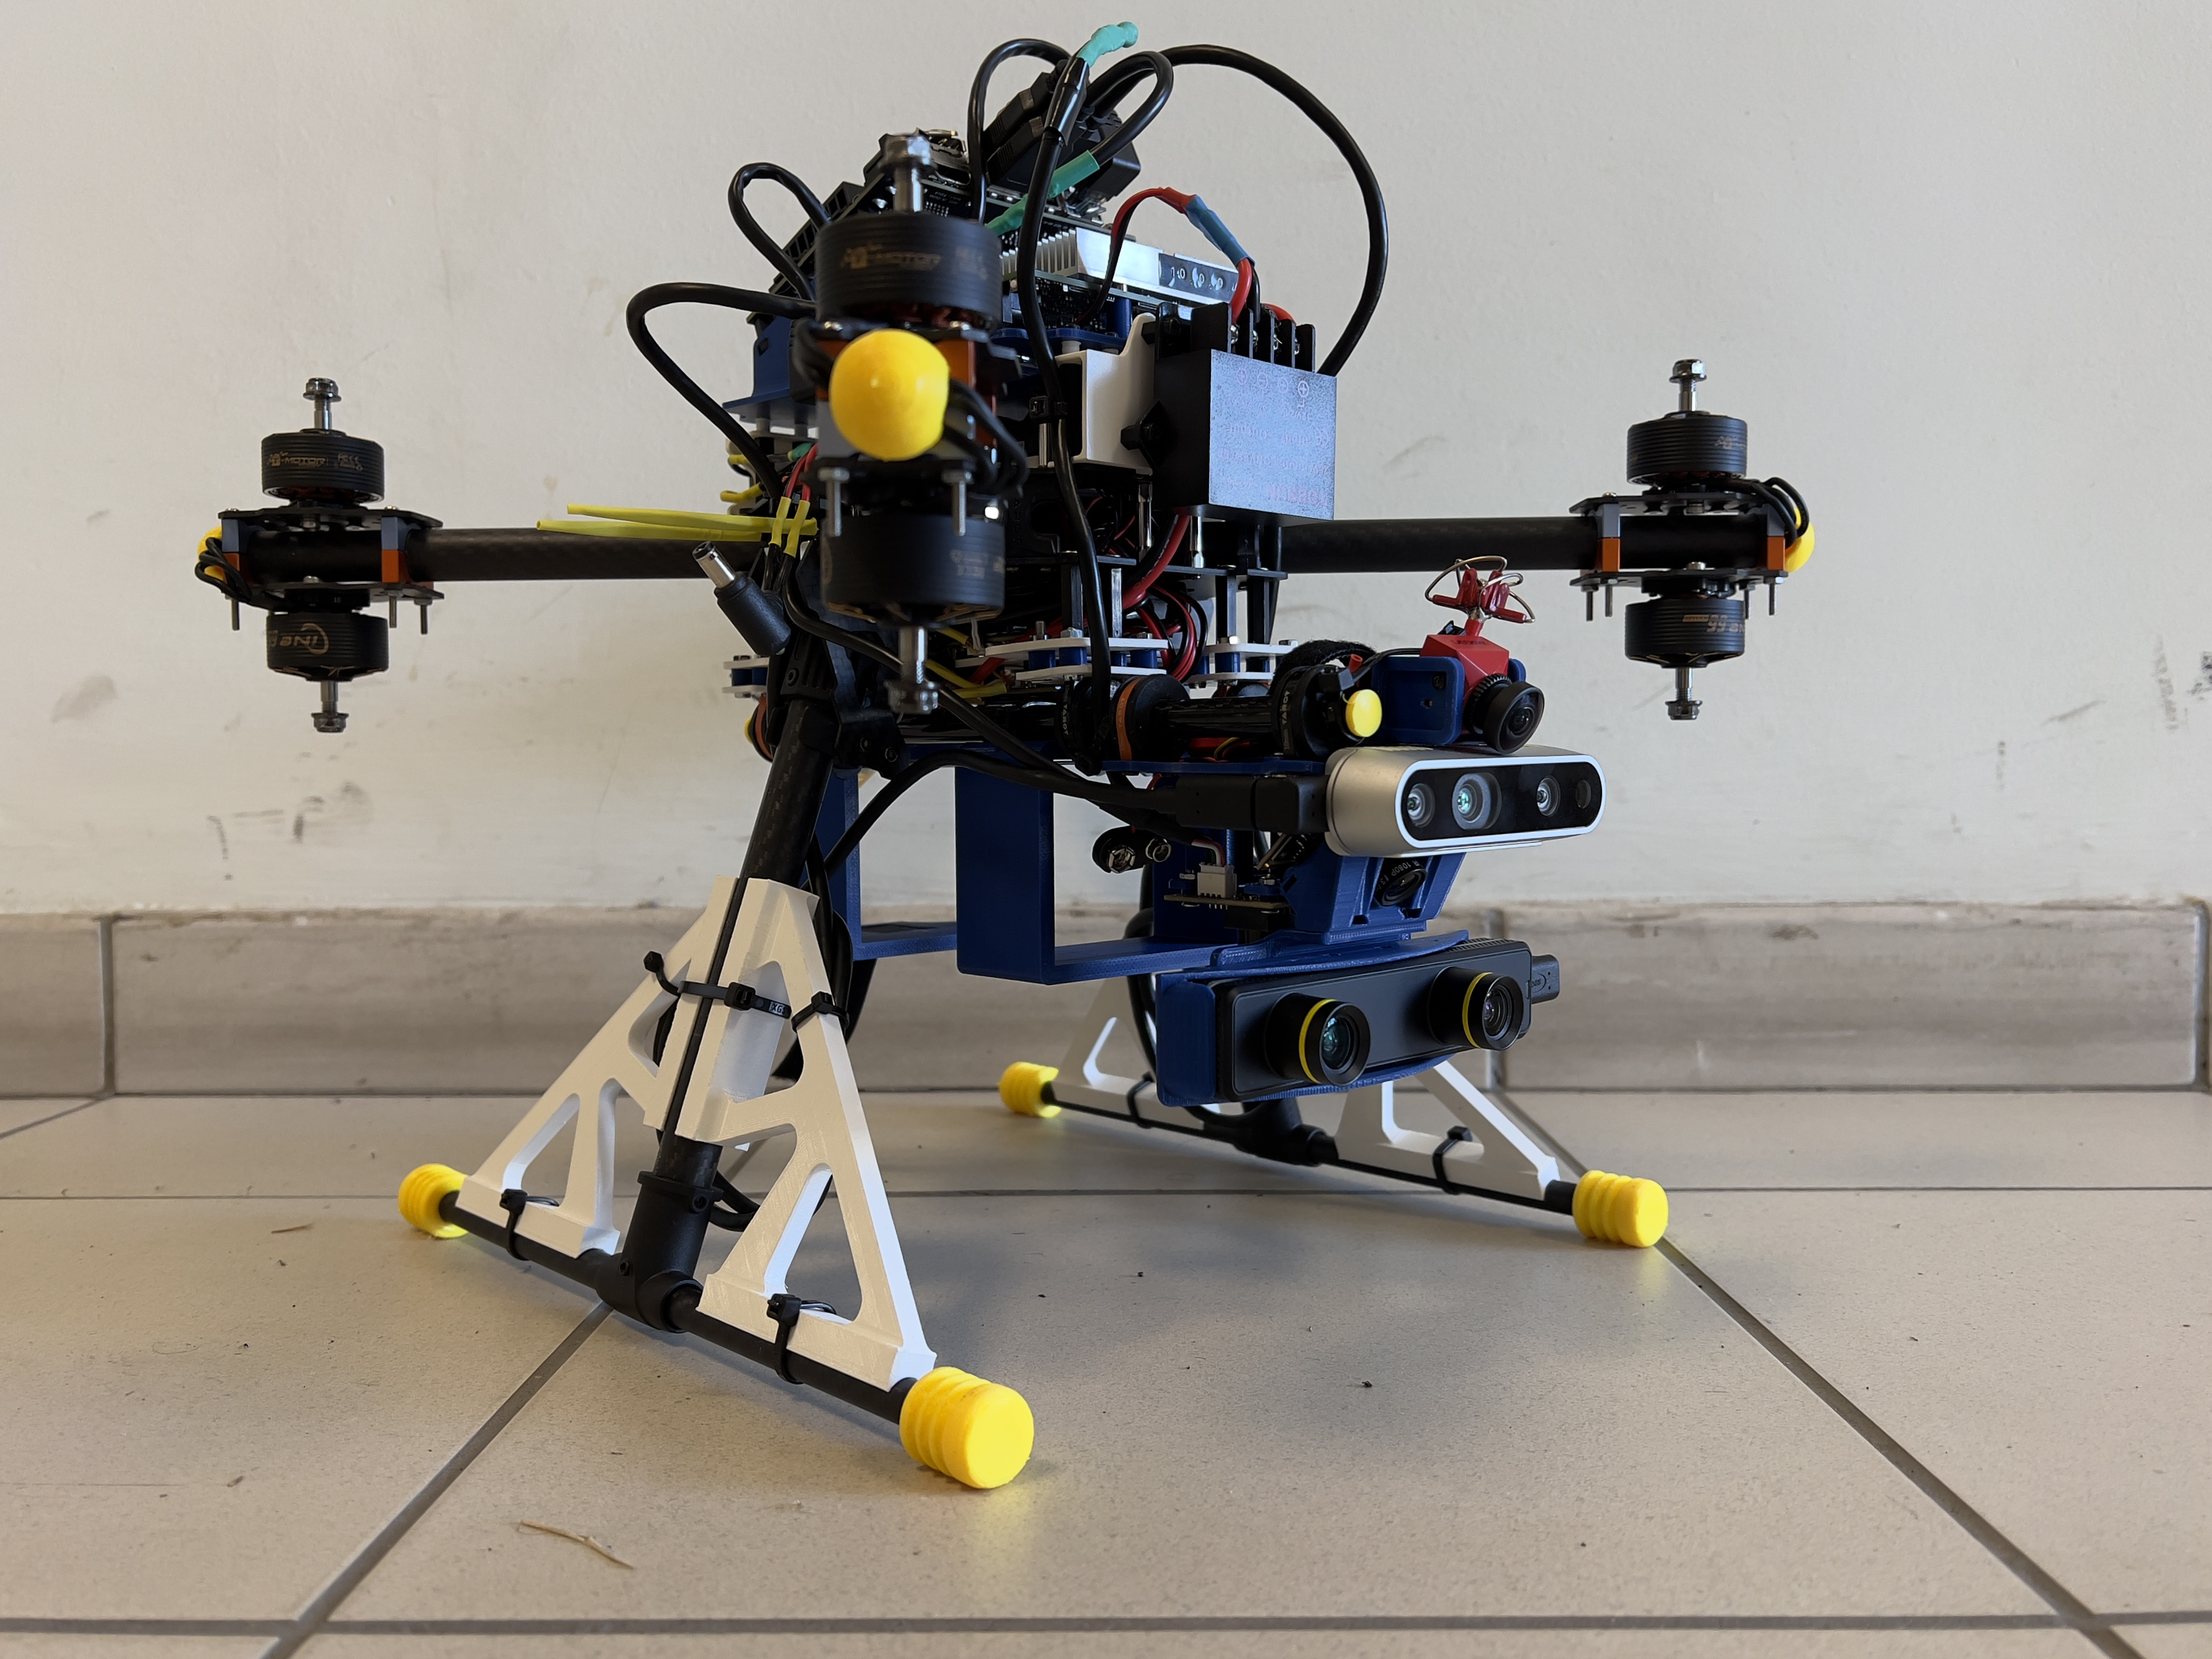
\includegraphics[width=.8\textwidth]{stanis}
			\caption{Stanis autonomous drone prototype.}
			\label{fig:stanis}
		\end{figure}
	\end{columns}
\end{frame}
\begin{frame}{The roboticist}{A new path for control engineers}
	\begin{columns}
		\column{.5\textwidth}
		A \textbg{roboticist} can usually:
		\begin{itemize}
			\item \textbg{design} solutions to complex problems;
			\item \textbg{develop} parts of a robot, or entire \textbg{control architectures};
			\item \textbg{deploy} and test software and hardware solutions;
			\item make use of modern \textbg{hardware accelerators} and robotics-oriented hardware.
		\end{itemize}
		Industries are looking for roboticist for their \textbg{versatile skill set}.

		\column{.5\textwidth}
		\begin{figure}
			\centering
			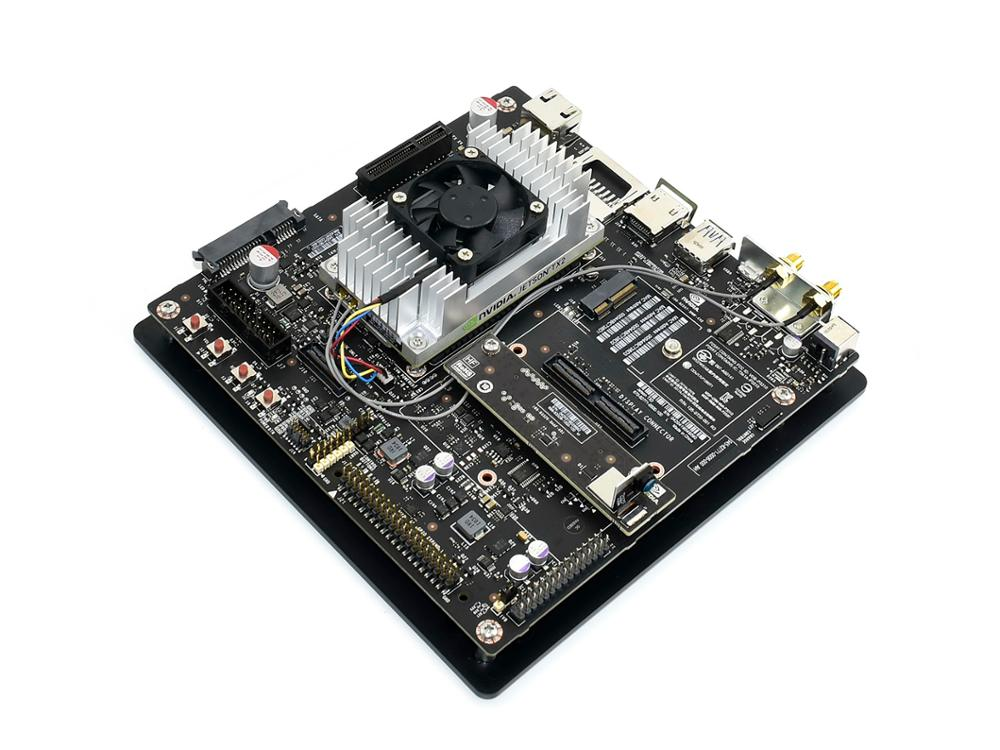
\includegraphics[width=.9\textwidth]{tx2}
			\caption{Nvidia Jetson TX2 developer kit.}
			\label{fig:tx2}
		\end{figure}
	\end{columns}
\end{frame}


% --- Section 2 ---
% Section 2 - Middleware in robotics
% Roberto Masocco <roberto.masocco@uniroma2.it>
% May 14, 2023

% ### Middleware in robotics ###
\section{Middleware in robotics}
\graphicspath{{figs/section2/}}

% --- What is middleware? ---
\begin{frame}{What is middleware?}
	\begin{figure}
		\centering
		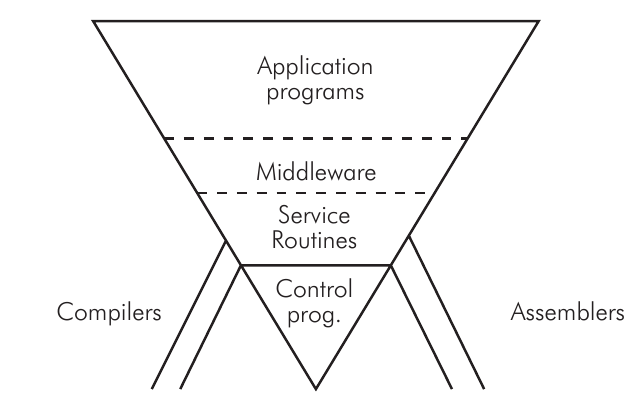
\includegraphics[width=.64\textwidth]{softwarePyramid.png}
		\caption{Software organization in a general-purpose computer system.}
		\label{fig:swpyramid}
	\end{figure}
\end{frame}
\begin{frame}{What is middleware?}
	\begin{block}{Definition of middleware}
		\justifying
		The term \textbf{middleware} identifies a kind of software that offers common services and functionalities to applications in addition to what an operating system usually does.
	\end{block}
	\justifying
	Middlewares are usually implemented as \textbg{libraries} that application programmers can use via appropriate \textbg{APIs}.
\end{frame}

% --- Middleware in robotics ---
\begin{frame}{Middleware in robotics}
	\justifying
	New problems arising when developing software for modern autonomous systems:
	\begin{itemize}
		\item integration of \textbg{sophisticated hardware} (microcontrollers, hardware accelerators, SBCs);
		\item \textbg{software} organization and maintenance;
		\item \textbg{communication} (involves both hardware and software!);
		\item debugging and \textbg{testing}.
	\end{itemize}
	\begin{block}{}
		\centering
		Middlewares can help to tackle and solve each one!
	\end{block}
\end{frame}

% --- Data Distribution Service ---
\begin{frame}{Data Distribution Service}
	\begin{block}{Definition of DDS}
		A DDS is a \textbf{publish-subscribe middleware} that handles communications between \textbf{real-time} systems and software over the network.
	\end{block}
	DDSs are currently used in automotive, aerospace, military...\\
	Their implementations follow an \textbg{open standard} that defines:
	\begin{itemize}
		\item \textbg{serialization} and \textbg{deserialization} of data packets (\texttt{RTPS Wire Protocol});
		\item \textbg{security protocols} and cryptographic operations;
		\item enforcing of \textbg{Quality of Service} policies to organize transmissions (specifying things like \textbg{queue sizes}, \textbg{best-effort} or \textbg{reliable} transmissions...);
	\end{itemize}
\end{frame}
\begin{frame}{Data Distribution Service}
	\begin{itemize}
		\item automatic discovery of \textbg{DDS participants} (over \textbg{multicast-IP/UDP}) and transmission of data (over \textbg{unicast-IP/UDP}) (\texttt{Discovery Protocol}).
	\end{itemize}
	\begin{figure}
		\centering
		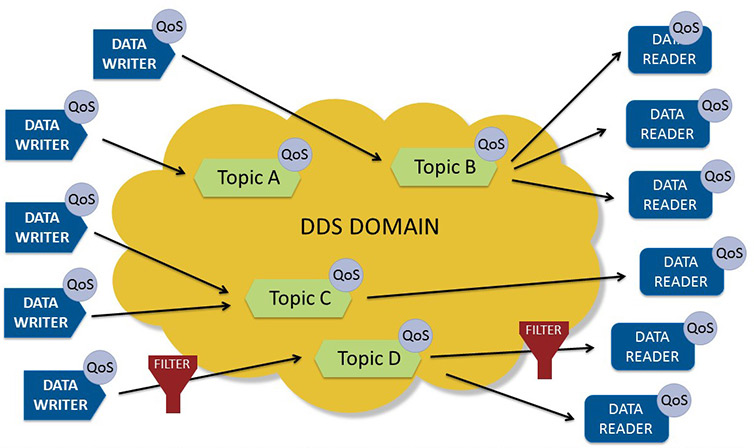
\includegraphics[scale=.32]{ddsDomain.jpg}
		\caption{Scheme of a DDS-based network (data space).}
		\label{fig:ddsdomain}
	\end{figure}
\end{frame}
\begin{frame}{Data Distribution Service}
	DDS participants can either \textbg{publish to} or \textbg{subscribe to} a \textbg{topic}.
	\begin{block}{Definition of DDS topic}
		A DDS topic is \textbf{uniquely identified} by three attributes:
		\begin{itemize}
			\item a \textbf{name}, \emph{i.e.}, a human-readable character string;
			\item an \textbf{interface}, \emph{i.e.}, a custom packet format that specifies what data is carried over it (\emph{e.g.}, strings, numbers, arrays...);
			\item a \textbf{QoS policy} that specifies how transmissions should be performed.
		\end{itemize}
	\end{block}
	\begin{block}{}
		\centering
		\textbf{Changing even only one of the above results in a completely different topic!}
	\end{block}
\end{frame}


% --- Section 3 ---
% Section 3 - ROS 2 overview
% Roberto Masocco <roberto.masocco@uniroma2.it>
% March 13, 2022

% ### ROS 2 overview ###
\section{ROS 2 overview}
\graphicspath{{figs/section3/}}

% --- What is ROS 2? ---
\begin{frame}{What is ROS 2?}
	\begin{columns}
		\column{.5\textwidth}
		\only<1>{
			\nolistindent ROS 2 is a \textbg{DDS-based}, \textbg{open-source} middleware for robotic applications.\\
      It allows developers to build and manage \textbg{distributed control architectures} made of many modules, usually referred to as \textbg{nodes}.
		}
		\only<2>{
			\nolistindent \nolistindent ROS 2 currently supports \textbg{C++} and \textbg{Python} for application programming, and runs natively on \textbg{Ubuntu Linux 22.04}.
      \newline\newline
			New versions are periodically released as \textbg{distributions}: the current LTS one is \textbg{Humble Hawksbill}; the development version is \textbg{Rolling Ridley} and can only be compiled from source.\\
      It is available as \textbg{binary \texttt{deb} packages} for \texttt{x86} and \texttt{ARMv8} architectures.
      \newline\newline
      A \textbg{distribution} is a collection of software packages: \textbg{libraries}, \textbg{tools}, and \textbg{applications}.
		}

		\column{.5\textwidth}
		\begin{figure}
			\centering
			
\includegraphics[width=.8\textwidth]{ros2Logo.jpg}
			\caption{ROS 2 logo.}
			\label{fig:ros2logos}
		\end{figure}
	\end{columns}
\end{frame}

% --- Why ROS 2? ---
\begin{frame}{Why ROS 2?}
	\begin{columns}
		\column{.5\textwidth}
    The ROS project started in 2007, to provide a middleware that could solve the \textbg{software integration} and \textbg{communication} problems in robotics. It has evolved much since then.
    \newline\newline
		ROS 2 helps to design and build \textbg{distributed control architectures}, providing a common ground for the \textbg{integration} of different systems, sensors, actuators, and algorithms.\\
    It is a common framework for the development of \textbg{robotics software}.
    \newline\newline
    Its adoption is still limited because of familiarity with the original ROS, but it is \textbg{growing}.

		\column{.5\textwidth}
		\begin{figure}
			\centering
      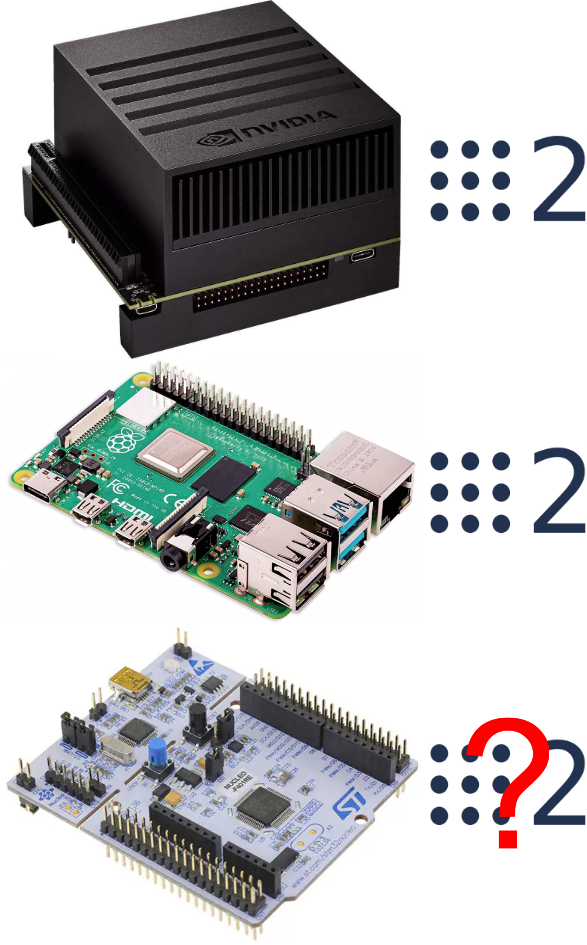
\includegraphics[scale=.17]{why_ros2.png}
      \label{fig:whyros2}
      \caption{STM32 (bottom), Raspberry Pi (middle), and Nvidia Xavier AGX (top).}
		\end{figure}
	\end{columns}
\end{frame}

% --- Main Features ---
\begin{frame}{Main features}
	As a middleware, it offers many \textbg{services to roboticists}, including:
	\begin{itemize}
		\item \textbg{three communication paradigms}, easy to set up and based on the DDS: \textbg{messages}, \textbg{services} and \textbg{actions};
		\item organization of software packages, allowing for \textbg{redistribution and code reuse}, thanks to the \textbg{\texttt{colcon}} package manager;
		\item module configuration tools: \textbg{node parameters} and \textbg{launch files};
		\item integrated \textbg{logging subsystem} (involves both console and log files);
		\item CLI \textbg{introspection tools} for debugging and testing;
	\end{itemize}
\end{frame}
\begin{frame}{Main features}
  \begin{itemize}
    \item may be integrated in some \textbg{simulators} (\emph{e.g.}, Gazebo) and \textbg{visualizers} (\emph{e.g.}, RViz).
  \end{itemize}
  \begin{figure}
    \centering
    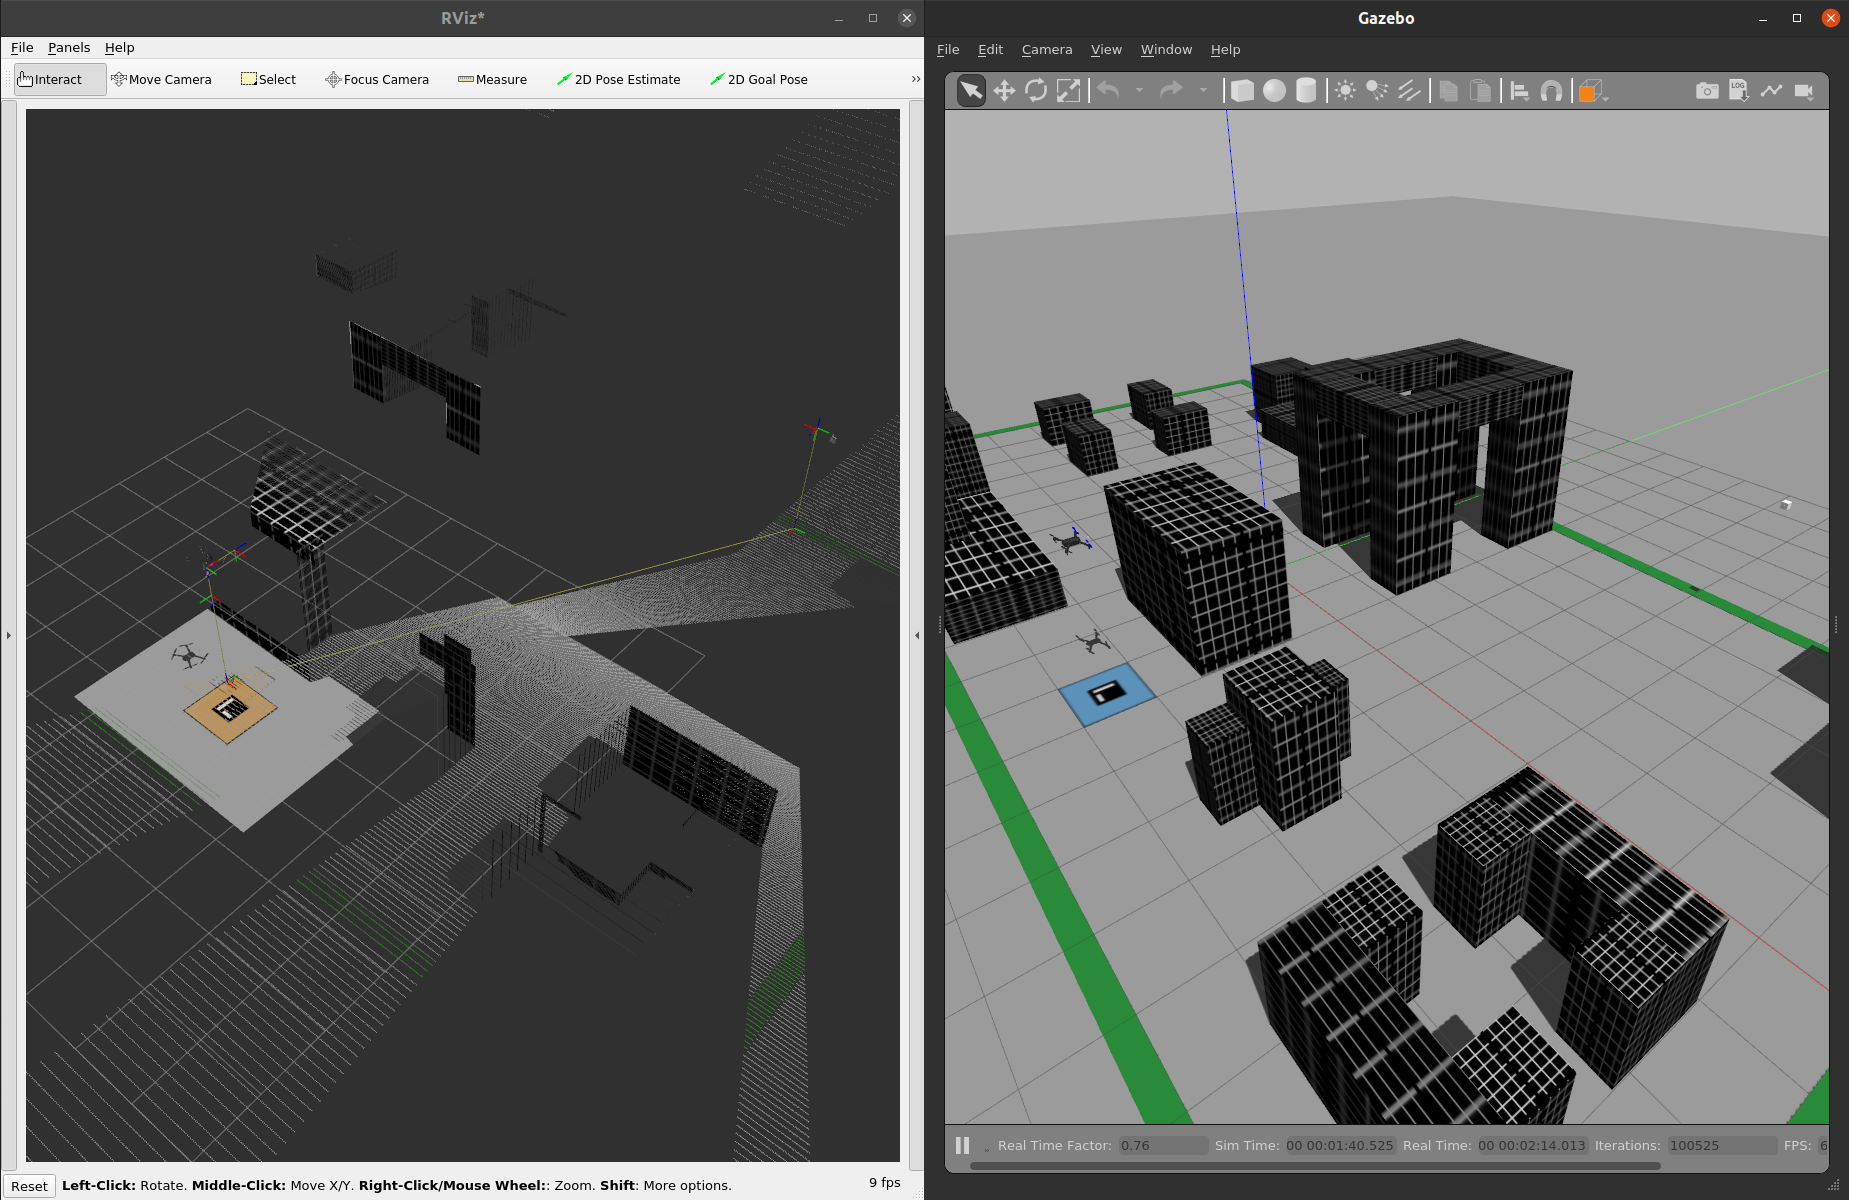
\includegraphics[scale=.133]{simulation.png}
    \label{fig:sim}
    \caption{Simulated drone in Gazebo Classic and RViz.}
  \end{figure}
\end{frame}

% --- Application Programming Interface ---
\begin{frame}{Application Programming Interface}{Deep dive into ROS 2 internals}
  A \textbg{ROS 2 installation}, from bottom to top, works as follows:
  \begin{enumerate}
    \item \textbg{DDS}: the middleware that implements the \textbg{communication layer} (many different implementations are supported).
    \item \textbg{RMW}: ROS MiddleWare, is the \textbg{DDS abstraction layer}, which allows to use different DDS implementations without changing the application code.
    \item \textbg{rcl}: ROS Client Support Library (C), implements basic entities: \textbg{nodes}, \textbg{publishers}, \textbg{subscribers}, \textbg{services}, \textbg{clients}, and \textbg{timers}.
    \item \textbg{rclc}/\textbg{rclcpp}/\textbg{rclpy}: ROS Client Library (C/C++/Python), implements the same entities as \texttt{rcl}, plus extended functionalities like the \textbg{executor}: a job scheduler.
  \end{enumerate}
  Then, there are \textbg{packages}: libraries, tools, and applications, both officially provided and community-contributed.
\end{frame}
\begin{frame}{Application Programming Interface}{How a ROS 2 application works}
  The most important entity is the \textbg{node}, whose functionalities are specified upon creation.

  A node must usually do \textbg{a single thing}, being the \textbg{unit} in a \textbg{distributed architecture}.

  With its class methods, it can:
  \begin{itemize}
    \item act as an \textbg{entry point} towards the DDS layer, to handle communications;
    \item embed \textbg{software modules} like data, algorithms, and threads, that implement the application logic;
    \item register \textbg{callbacks} to handle \textbg{events}, such as timers or incoming messages.
  \end{itemize}
  Thus, it is both an \textbg{operational unit} and a \textbg{communication endpoint}.

  Nodes are usually handled by \textbg{executors}, which are responsible for scheduling and processing their workload.

  \begin{alertblock}{}
    \centering
    \textbr{Nodes are just objects in your application: they can embed any kind of software module, but they do not limit the design to their paradigms.}
  \end{alertblock}
\end{frame}

% --- Executors: events and callbacks ---
\begin{frame}{Executors}{Handling events and callbacks}
	\begin{figure}
		\centering
		\includesvg[scale=.45]{ROS2_executor_scheme.svg}
		\label{fig:executorscheme}
		\caption{ROS 2 event-based programming paradigm.}
	\end{figure}
\end{frame}
\begin{frame}{Executors}{Handling events and callbacks}
	\begin{enumerate}
		\item Middleware functionalities trigger \textbg{(a)synchronous events}.
		\item Events are handled by \textbg{background jobs}, coded in \textbg{callbacks} by the programmer.
		\item Callbacks are \textbg{registered} into a \textbg{node} when its functionalities are specified (\emph{e.g.}, upon creation).
		\item The workload that a node carries is scheduled and processed by an \textbg{executor}, single- or multi-threaded.
	\end{enumerate}
	\begin{alertblock}{}
    \centering
		Executors implement a \textbr{round-robin}, \textbr{non-preemptive} policy that \textbr{always prioritizes timers}.
	\end{alertblock}
\end{frame}

% --- Flaws ---
\begin{frame}{Flaws}
	\visible<1->{
		\begin{alertblock}{ROS 2 biggest flaws (as of today)}
			The main concerns arise when developing low-level stuff:
			\begin{itemize}
				\item \textbr{the DDS layer is almost completely abstracted}, so non-standard network configurations may get tricky;
				\item the internal job scheduling algorithm (namely the \textbr{executor}) is \textbr{not suited for hard real-time applications} because of its \textbr{non-preemptive} nature.
			\end{itemize}
		\end{alertblock}
	}
	\visible<2>{
		What to do when development gets to a really low level?
		\begin{itemize}
			\item Use something else.
			\item Hand off stuff to dedicated \textbg{microcontrollers}.
			\item Use \textbg{micro-ROS}: hard real-time ROS 2 on microcontrollers and different communication interfaces.
		\end{itemize}
	}
\end{frame}


% --- Section 4 ---
% Section 4 - Containers
% Roberto Masocco <roberto.masocco@uniroma2.it>
% May 14, 2023

% ### Containers ###
\section{Containers}
\graphicspath{{figs/section4/}}

% --- Why containers? ---
\begin{frame}{Why containers?}
	\begin{exampleblock}{Example: Packaging applications}
		Suppose you are ready to distribute your new application:
		\begin{itemize}
			\item you need to be sure that it is compatible with all the \textbf{platforms} you chose to support;
			\item you need to figure out a way to deal with \textbf{dependencies};
			\item you want to publish some kind of \textbf{self-contained}, easily-identifiable \textbf{package}.
		\end{itemize}
	\end{exampleblock}
\end{frame}
\begin{frame}{Why containers?}
	\begin{exampleblock}{Example: Isolating applications}
		Suppose you are deploying applications on a server:
		\begin{itemize}
			\item you want to define \textbf{resource quotas} and \textbf{permissions} for each;
			\item you want to be sure that each module has what it needs to operate, but \textbf{nothing more};
			\item you want to \textbf{isolate} each module for security reasons, in case something goes wrong.
		\end{itemize}
	\end{exampleblock}
\end{frame}
\begin{frame}{Why containers?}
	\begin{exampleblock}{Example: Replicating environments}
		Suppose you are developing applications for a specific system (maybe with a different architecture):
		\begin{itemize}
			\item you want to have a \textbf{software copy} of such system without having to carry it with you;
			\item you want to have all \textbf{libraries} and \textbf{dependencies} installed without tainting your own;
			\item you would like to \textbf{deploy} the entire installation with just a few commands.
		\end{itemize}
	\end{exampleblock}
\end{frame}
\begin{frame}{Why containers?}
	\begin{columns}
		\column{.5\textwidth}
		A possible solution to many of the previous situations could be a set of \textbg{virtual machines}.\\
		However, virtual machines are \textbg{slow}, hypervisors take up \textbg{system resources} and guest kernels must always be \textbg{tweaked}.
		\newline\newline
		In each of the above scenarios something simpler would be enough, especially since \textbg{the OS is not involved}, only applications are.
		\begin{block}{}
			\centering
			This is what a \textbf{container} is.
		\end{block}

		\column{.5\textwidth}
		\begin{figure}
			\centering
			
\includegraphics[scale=.7]{freebsdjail.png}
			\label{fig:jail}
			\caption{FreeBSD jail logo.}
		\end{figure}
	\end{columns}
\end{frame}

% --- Containers in the Linux kernel ---
\begin{frame}{Containers in the Linux kernel}
	\begin{columns}
		\column{.5\textwidth}
		Support for containers was added to the Linux kernel with a set of \textbg{features} starting from kernel 2.6 (2003), mainly:
		\begin{itemize}
			\item \textbg{control groups} (\texttt{cgroups}): defining different resource usage policies for groups of processes;
			\item \textbg{namespaces}: isolating processes and users in different "realms", both hardware (e.g. network stack) and software (e.g. PIDs);
			\item \textbg{capabilities}: granting some of the superuser's permissions to unprivileged threads.
		\end{itemize}

		\column{.5\textwidth}
		\begin{figure}
			\centering
			
\includegraphics[scale=.2]{tux.png}
			\label{fig:tux}
			\caption{Tux.}
		\end{figure}
	\end{columns}
\end{frame}
\begin{frame}{Containers in the Linux kernel}
	\begin{figure}
		\centering
		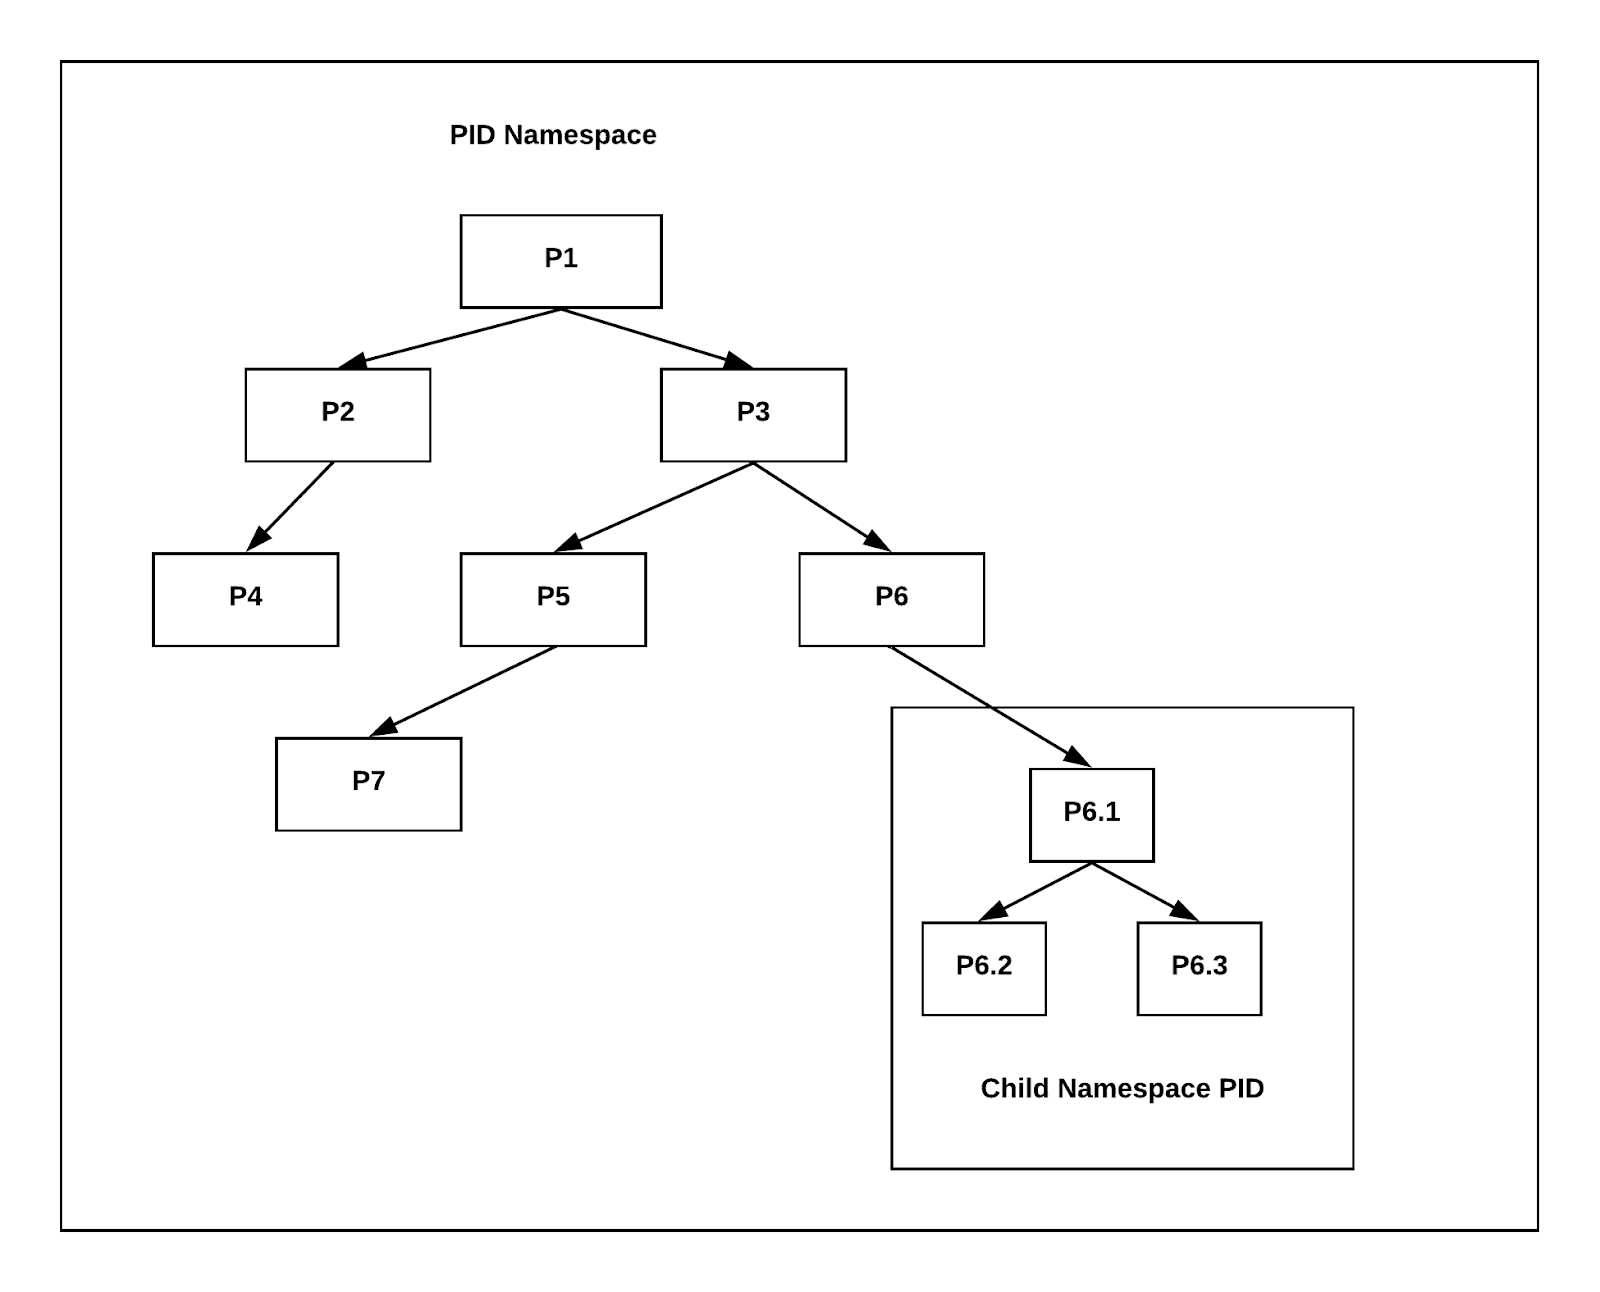
\includegraphics[scale=.137]{pidNamespace.png}
		\label{fig:pidnamespace}
		\caption{Nested PID namespaces.}
	\end{figure}
\end{frame}


% --- Section 5 ---
% Section 5 - Docker
% Roberto Masocco <roberto.masocco@uniroma2.it>
% May 17, 2023

% ### Docker ###
\section{Docker}
\graphicspath{{figs/section5/}}

% --- Docker Engine ---
\begin{frame}{Docker Engine}
	\begin{columns}
		\column{.5\textwidth}
		\textbg{Docker} is the currently de-facto standard for building, managing and distributing \textbg{multiplatform} containers.
		\newline\newline
		It is an engine (\emph{i.e.}, a collection of \textbg{daemons}) that automates the management of the kernel subsystems in order to set up, store and run containers.

		\column{.5\textwidth}
		\begin{figure}
			\centering
			\label{fig:docker}
			
\includegraphics[scale=.2]{docker.png}
			\caption{Docker logo.}
		\end{figure}
	\end{columns}
\end{frame}
\begin{frame}{Docker Engine}
	\begin{figure}
		\centering
		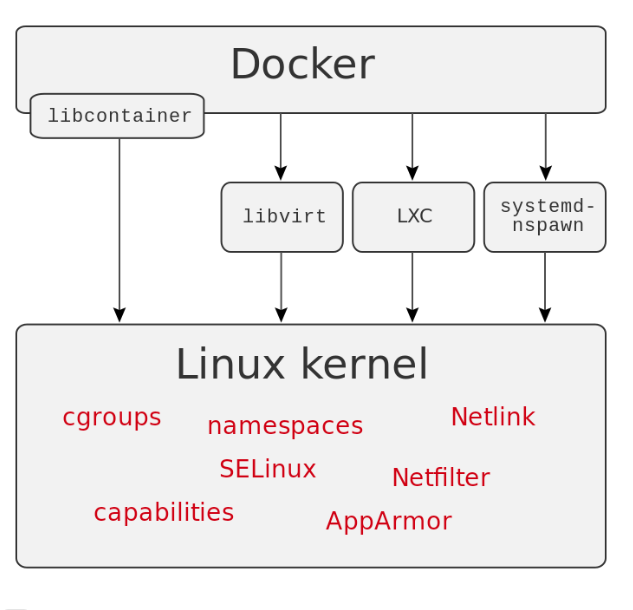
\includegraphics[scale=.29]{dockerScheme.png}
		\label{fig:dockerscheme}
		\caption{Docker Engine scheme.}
	\end{figure}
\end{frame}

% --- Containers in robotics ---
\begin{frame}{Containers in robotics}
	Containers can be of help in some classic scenarios:
	\begin{itemize}
		\item \textbg{deploying} applications or whole control architectures, solving issues like \textbg{dependencies} and \textbg{configurations};
		\item configuring and distributing \textbg{development environments};
		\item working with \textbg{multiple architectures} at the same time: Docker fully supports \href{https://www.qemu.org/}{\color{blue}\textbf{\underline{QEMU}}} to build and run containers;
		\item expanding the capabilities of \textbg{(partially) closed-source} hardware solutions (\emph{e.g.}, Nvidia Jetson...).
	\end{itemize}
\end{frame}

% --- Building a Docker container ---
\begin{frame}{Building a Docker container}{Step by step}
	\begin{enumerate}
		\item A \textbg{Dockerfile} specifies a set of rules to build an \textbg{image}, just like a script.
		\item \textbg{Images} are the binary archives from which a \textbg{container} can be started: they can be stored, pulled from a remote \textbg{registry} or simply built locally.
		\item A \textbg{container} can be built from an image and then started, stopped and managed by the Docker daemon.
		\item Processes started inside the container are subject to its limitations, \emph{e.g.}, \textbg{filesystem jails} prevent them to climb up to the hosts's filesystem.
	\end{enumerate}
	Images are built \textbg{incrementally}: each Dockerfile directive defines a new \textbg{layer}, and the Docker engine stores the differences between each build step thanks to \textbg{OverlayFS}.\\
	For every new container, its filesystem will be in a \textbg{new top layer}.\\
	This allows to efficiently \textbg{cache and share build stages}, which will then be stacked together to form images, but operating in a \textbg{copy-on-write}, \textbg{slower} fashion.
\end{frame}

% --- Dockerfiles ---
\begin{frame}[fragile]{Dockerfiles}
	\begin{columns}\column{.9\textwidth}
		\begin{lstlisting}[language=Dockerfile, caption=Minimal example of a Dockerfile running an Ubuntu image in a container.]
ARG VERSION=22.04
FROM ubuntu:$VERSION # Note the tag!

ENV DEBIAN_FRONTEND=noninteractive

RUN apt-get update && \
    apt-get install -y --no-install-recommends \
    build-essential \
    git && \
    rm -rf /var/lib/apt/lists/* /tmp/* /var/tmp/*/apt/lists/*

ENV DEBIAN_FRONTEND=dialog
LABEL maintainer.name="Roberto Masocco"
CMD ["bash"]
\end{lstlisting}
	\end{columns}
\end{frame}

% --- Dockerfile commands ---
\begin{frame}{Dockerfile commands}
	\begin{itemize}
		\item \texttt{FROM repository/image:tag}\\Specifies a base image to pull.
		\item \texttt{RUN command}\\Runs the following command in a new shell inside the container.
		\item \texttt{COPY source target}\\Copies a file into the container.
		\item \texttt{ENV variable=value}\\Sets an environment variable inside the container.
		\item \texttt{ARG name=value}\\Declares a build argument.
		\item \texttt{CMD ["command", "arg1", ...]}\\Specifies the command to run when the container is started.
	\end{itemize}
\end{frame}

% --- Docker commands ---
\begin{frame}{Docker commands}
	Again, just a few (each with a gazillion of options):
	\begin{itemize}
		\item \texttt{docker build}\\Builds a new image from a Dockerfile.
		\item \texttt{docker run}\\Builds and starts a container.
		\item \texttt{docker ps}\\Lists active containers.
		\item \texttt{docker exec}\\Runs a command inside a container (\emph{e.g.}, a shell).
		\item \texttt{docker start}\\Starts a container.
	\end{itemize}
\end{frame}
\begin{frame}{Docker commands}
	\begin{itemize}
		\item \texttt{docker stop}\\Stops a container.
		\item \texttt{docker images}\\Lists available images.
		\item \texttt{docker rm}\\Removes a container.
		\item \texttt{docker rmi}\\Removes an image.
	\end{itemize}
	Active containers are usually referenced by their \textbg{ID} (\emph{e.g.}, \texttt{abae6cae4648}).
	\newline\newline
	See the \href{https://docs.docker.com/engine/reference/builder/}{\color{blue}\underline{Dockerfile reference}} and the \href{https://docs.docker.com/engine/reference/commandline/docker/}{\color{blue}\underline{Docker CLI reference}} for more.
\end{frame}

% --- Containers on real robots ---
\begin{frame}{Containers on real robots}{Best practices}
  To run containers on embedded systems and robot SBCs, some configurations are suggested which \textbg{would not apply} in traditional containerization scenarios:
  \begin{itemize}
    \item the host \textbg{network stack} should be fully exposed to allow for \textbg{ROS} and other network-based \textbg{middleware} to work properly (\texttt{-{}-network host});
    \item the \textbg{IPC namespace} should be shared to allow for \textbg{shared memory} and \textbg{IPC} to work properly (\texttt{-{}-ipc host});
    \item to allow access to the \textbg{hardware} mounted on the host, one should grant full privileges to the container (\texttt{-{}-privileged}) and mount \texttt{/dev} and \texttt{/sys} inside it (\texttt{-v /dev:/dev -v /sys:/sys});
    \item your development directory should be \textbg{mounted as a volume} inside the container, so that file manipulations happen on the host filesystem (\texttt{-v /your/code:/workspace}).
  \end{itemize}
  We would like some utility to \textbg{automate} this process...
\end{frame}


% --- Section 6 ---
%% Section 6 - Docker Compose
% Roberto Masocco <roberto.masocco@uniroma2.it>
% May 17, 2022

% ### Docker Compose ###
\section{Docker Compose}
\graphicspath{{figs/section6/}}

% --- Composing services ---
\begin{frame}{Composing services}
	\begin{columns}
		\column{.5\textwidth}
		Managing multiple, interdependent \textbg{containerized services} can become quite a tedious task.
    \newline\newline
		Each container may take multiple options, some have to be started in sequence or built in a particular way...
		\begin{block}{}
			\centering
			\textbf{Compose} is a utility that helps to \textbf{build}, \textbf{run} and \textbf{manage} multiplatform containers by parsing all such settings from \textbf{YAML configuration files}.
		\end{block}
    For instance, \textbg{our code repository} cointains development containers managed by Compose.

		\column{.5\textwidth}
		\begin{figure}
			\centering
			
\includegraphics[scale=.25]{composeLogo.png}
			\label{fig:compose}
			\caption{Docker Compose logo.}
		\end{figure}
	\end{columns}
\end{frame}

% --- Compose files ---
\begin{frame}[fragile]{Compose files}
	\begin{columns}\column{.9\textwidth}
		\begin{lstlisting}[language=compose, caption=Minimal example of a Compose file.]
services:
  development:
    build:
      context: .
      args:
        TARGET: dev
    image: devenv:latest
    environment:
      TERM: xterm-256color
    network_mode: host
    command: ["/bin/zsh"]
    volumes:
      - ~/.ssh:/home/user/.ssh
\end{lstlisting}
	\end{columns}
	Refer to the \href{https://docs.docker.com/compose/compose-file/}{\color{blue}\underline{Compose reference}} for more.
\end{frame}

% --- Compose commands ---
\begin{frame}{Compose commands}
	Pretty much the same that Docker has, but invoked with
  \newline\newline
	\texttt{docker-compose}
  \newline\newline
	instead of \texttt{docker}, and oriented only towards services specified in the local Compose file.
  \newline\newline
	See the \href{https://docs.docker.com/compose/reference/}{\color{blue}\underline{Compose CLI reference}} for more.
\end{frame}


\end{document}
